\documentclass[a4paper,11pt,titlepage]{article}

\usepackage{ucs}
% per input encoding kann man Umlaute direkt einsetzten, aber  dann ist man von Font des jeweiligen Rechners abh"angig. Daher mag ich es nicht!
%\usepackage[utf8x]{inputenc}
\usepackage[german,ngerman]{babel}
\usepackage{fontenc}
\usepackage[pdftex]{graphicx}
%\usepackage{latexsym}

\usepackage[pdftex]{hyperref}

\begin{document}

% hier aktuelle Uebungsnummer einfuegen
    \title{Einf\"uhrung in die Informatik\\
    Ausarbeitung \"Ubung 0}

% Namen der Bearbeiter einfuegen

    \author{Tim Zolleis}

% aktuelles Datum einfuegen

    \date{\today}

    \maketitle{\thispagestyle{plain}}


    \section{Aufgabe 1 - Einf"uhrung in \LaTeX}

    \subsection{Der folgende Satz enth"alt ein hohes Maß an Umlauten:}

    "Uberm"aßiges Gl"uck f"uhrt zu "uberm"aßigem L"acheln, w"hrend der V"ogel im Fr"uhling fr"ohlich zwitschern.

    \subsection{Abs"atze}
    hier ist Text \\

    Dann kommt ein neuer Absatz\newline

    \noindent und dieser hier auch (aber ohne Einr\"ucken)

    \subsection{Listen}

    Dies ist ein Beispiel einer einfachen Liste:
    \begin{itemize}
        \item Eintrag 1
        \item Eintrag 2
        \item Eintrag 3
    \end{itemize}

    \noindent Hier ein Beispiel einer nummerierten Liste:
    \begin{enumerate}
        \item Eintrag 1
        \item Eintrag 2
        \item Eintrag 3
    \end{enumerate}

    \noindent Und zum Schluss noch eine Liste mit mehreren Ebenen
    \begin{itemize}
        \item Ebene 1
        \begin{itemize}
            \item Ebene 2
            \begin{itemize}
                \item Ebene 3
            \end{itemize}
        \end{itemize}
    \end{itemize}

    \subsection{Tabellen}
    Tabellen sind etwas interessanter in LaTeX. Hier einmal eine Tabelle mit "Uberschrift

    \begin{center}
        \begin{tabular}{ | l | p{5 cm} |}
            \hline
            Substanz & Dichte  \\ \hline
            "Ol      & .8 g/mL \\ \hline
            "Ol      & .8 g/mL \\ \hline
            "Ol      & .8 g/mL \\ \hline
        \end{tabular}
    \end{center}

    \subsection{Bilder}
    \begin{figure}
        \centering
        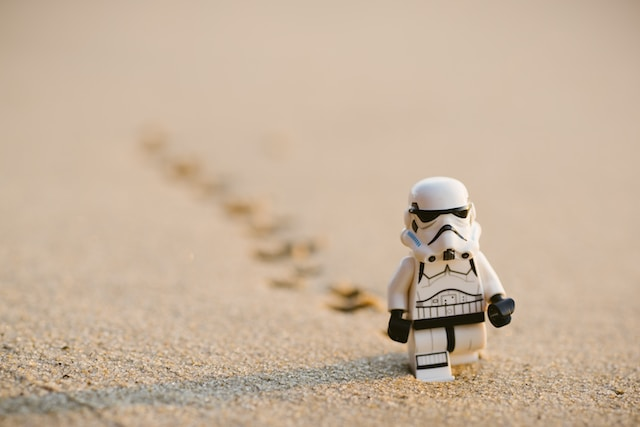
\includegraphics[width=8cm]{./images/start-wars-desert}
        \caption{Storm trooper wandering in the desert}
        \label{fig:star-wars}
    \end{figure}
\end{document}
